\documentclass[12pt, a4paper, oneside]{book}
\usepackage[hidelinks]{hyperref}
\usepackage[slovak]{babel}
\usepackage{epsfig}
\usepackage{epstopdf}
\usepackage[chapter]{algorithm}
\usepackage{algorithmic}
\usepackage{listings}
\usepackage{amsmath}
\usepackage{amssymb}
\usepackage{graphicx}
\usepackage{multirow}
\usepackage{color}
\usepackage{url}
\usepackage[utf8]{inputenc}
\usepackage[T1]{fontenc}
\usepackage{setspace}
\usepackage{tabularx}
\usepackage{textcomp}
\usepackage{caption}
\usepackage{subcaption}
\usepackage{natbib}
\usepackage[avantgarde]{quotchap}

%obrazok
\newcommand{\obrazok}[1]{(Obr.  \ref{#1})}
\newcommand{\tabulka}[1]{(Tabuľka  \ref{#1})}

\usepackage{listings}
\usepackage{color}
\definecolor{lightgray}{gray}{0.9}

\lstset{
    showstringspaces=false,
    basicstyle=\ttfamily,
    keywordstyle=\color{blue},
    commentstyle=\color[grey]{0.6},
    stringstyle=\color[RGB]{0,150,0},
    literate=%
    {á}{{\'a}}1
    {ä}{{\"a}}1
    {č}{{\v{c}}}1
    {ď}{{\v{d}}}1
    {é}{{\'e}}1
    {ě}{{\v{e}}}1
    {í}{{\'i}}1
    {ľ}{{\v{l}}}1
    {ĺ}{{\'{l}}}1
    {ň}{{\v{n}}}1
    {ó}{{\'o}}1
    {ř}{{\v{r}}}1
    {š}{{\v{s}}}1
    {ť}{{\v{t}}}1
    {ú}{{\'u}}1
    {ů}{{\r{u}}}1
    {ý}{{\'y}}1
    {ž}{{\v{z}}}1
    {Á}{{\'A}}1
    {Ä}{{\"A}}1
    {Č}{{\v{C}}}1
    {Ď}{{\v{D}}}1
    {É}{{\'E}}1
    {Ě}{{\v{E}}}1
    {Í}{{\'I}}1
    {Ľ}{{\v{L}}}1
    {Ĺ}{{\'{L}}}1
    {Ň}{{\v{N}}}1
    {Ó}{{\'O}}1
    {Ř}{{\v{R}}}1
    {Š}{{\v{S}}}1
    {Ť}{{\v{T}}}1
    {Ú}{{\'U}}1
    {Ů}{{\r{U}}}1
    {Ý}{{\'Y}}1
    {Ž}{{\v{Z}}}1
}
\newcommand{\inlinecode}[2]{\colorbox{lightgray}{\lstinline[language=#1]$#2$}}
\newcommand{\inlinecodebase}[1]{\colorbox{lightgray}{\texttt{#1}}}
\setstretch{1.5}
%\renewcommand\baselinestretch{1.5} % riadkovanie jeden a pol

% pekne pokope definujeme potrebne udaje
\newcommand\mftitle{Klaboratívny grafický editor pre MediaWiki}
\newcommand\enmftitle{Collaborative graphics editor for MediaWiki}
\newcommand\mfthesistype{Diplomová práca}
\newcommand\enmfthesistype{Master thesis}
\newcommand\mfauthor{Bc. Martin Krasňan}
\newcommand\mfadvisor{doc. RNDr. Zuzana Kubincová, PhD.}
\newcommand\mfplacedate{Bratislava, 2018}
\newcommand\mfuniversity{UNIVERZITA KOMENSKÉHO V BRATISLAVE}
\newcommand\mffaculty{FAKULTA MATEMATIKY, FYZIKY A INFORMATIKY}
\newcommand\mfpracovisko{Katedra aplikovanej informatiky}
\newcommand\enmfpracovisko{Department of Applied Informatics}

\newcommand{\sub}[1]{$_{\text{#1}}$}
\newcommand{\reference}[1]{č.~\ref{#1}}
\newcommand{\imageHeight}{150px}

\ifx\pdfoutput\undefined\relax\else\pdfinfo{ /Title (\mftitle) /Author (\mfauthor) /Creator (PDFLaTeX) } \fi

\begin{document}

\frontmatter

\thispagestyle{empty}

\noindent
\begin{minipage}{\textwidth}
\begin{center}
\textbf{\mfuniversity \\
\mffaculty}
\end{center}
\end{minipage}

\vfill
\begin{figure}[!hbt]
	\begin{center}
		
\includegraphics{images/logo_fmph}
		\label{img:logo}
	\end{center}
\end{figure}
\begin{center}
	\begin{minipage}{0.8\textwidth}
		\centerline{\textbf{\Large\MakeUppercase{\mftitle}}}
		\smallskip
		\centerline{\mfthesistype}
	\end{minipage}
\end{center}
\vfill
2018 \hfill
\mfauthor
\eject 
% koniec obalu

\thispagestyle{empty}

\noindent
\begin{minipage}{\textwidth}
\begin{center}
\textbf{\mfuniversity \\
\mffaculty}
\end{center}
\end{minipage}

\vfill
\begin{figure}[!hbt]
\begin{center}

\includegraphics{images/logo_fmph_dark}
\label{img:logo_dark}
\end{center}
\end{figure}
\begin{center}
\begin{minipage}{0.8\textwidth}
\centerline{\textbf{\Large\MakeUppercase{\mftitle}}}
\smallskip
\centerline{\mfthesistype}
\end{minipage}
\end{center}
\vfill
\begin{tabular}{l l}
%Registration number: & 40a99bd8-3cb6-4534-9330-c7fd9b5e5ca4 \\
Študijný program: & Aplikovaná informatika\\
Študijný odbor: & 2511 Aplikovaná informatika\\
Školiace pracovisko: & Katedra aplikovanej informatiky\\
Školiteľ: & \mfadvisor
\end{tabular}
\vfill
\noindent
\mfplacedate \hfill
\mfauthor
\eject 
% koniec titulneho listu

%\thispagestyle{empty}
%\includegraphics[width=\textwidth]{images/zadanie}
%\vfill
%\eject
% koniec zadania

\thispagestyle{empty}


\begin{figure}[H]
\begin{center}
\makebox[\textwidth]{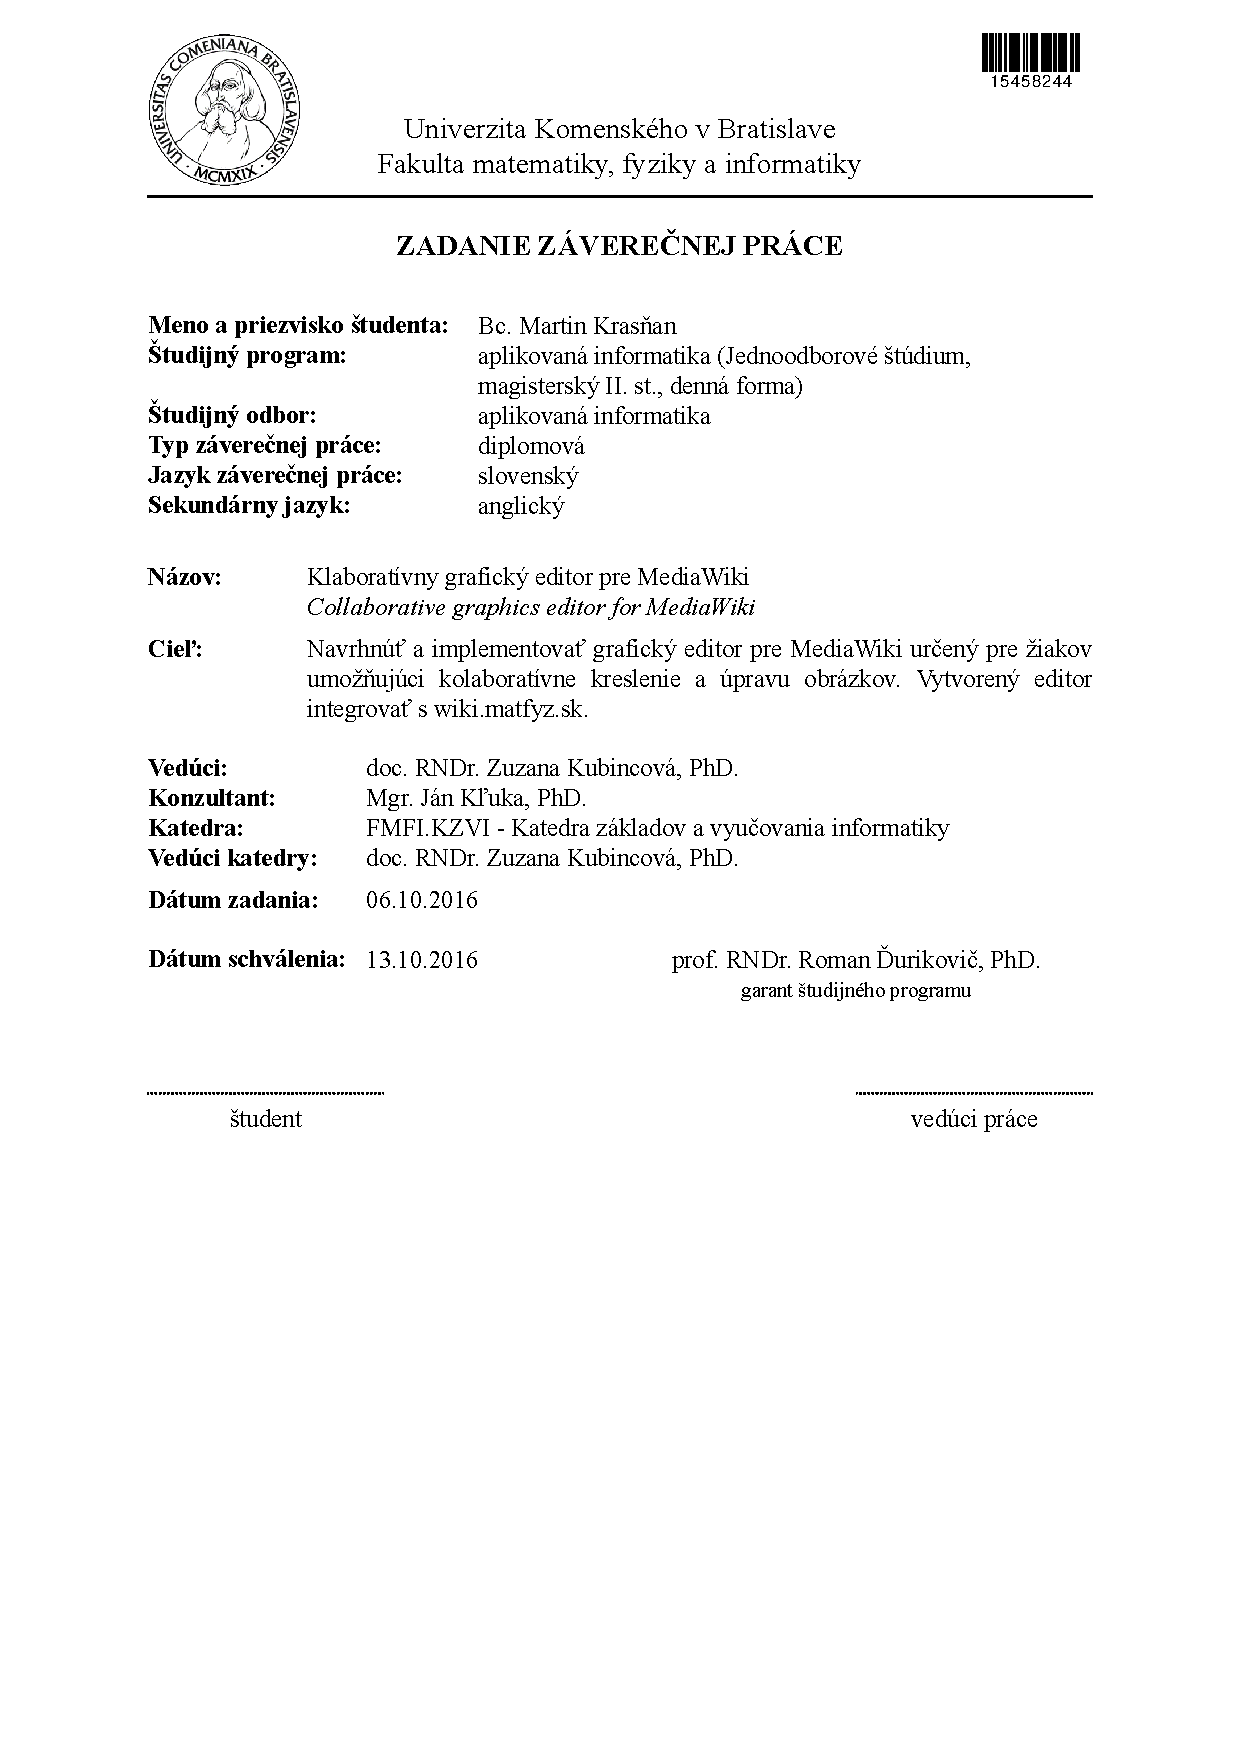
\includegraphics[width=\paperwidth]{images/zadaniedp}}
\label{img:zadanie}
\end{center}
\end{figure}

{~}\vspace{12cm}

\noindent
\begin{minipage}{0.25\textwidth}~\end{minipage}
\begin{minipage}{0.75\textwidth}
Čestne vyhlasujem, že som túto diplomovú prácu vypracoval samostatne pod vedením doc. RNDr. Zuzany Kubincovej, PhD., s použitím zdrojov uvedených v zozname použitej literatúry.
\newline \newline
\end{minipage}
\vfill
~ \hfill {\hbox to 6cm{\dotfill}} \\
\mfplacedate \hfill \mfauthor
\vfill\eject 
% koniec prehlasenia

\chapter*{Poďakovanie}\label{chap:thank_you}
...podakovanie...
\vfill\eject 
% koniec podakovania

\chapter*{Abstrakt}\label{chap:abstract_sk}
\MakeUppercase{Krasňan}, Martin: \textit{\mftitle} [\mfthesistype]. - Univerzita Komenského v Bratislave. Fakulta matematiky, fyziky a informatiky; \mfpracovisko. - Školiteľ: \mfadvisor. Bratislava: \mfplacedate. ?? strán.

Text abstraktu...

~\\
Kľúčové slová: klucove, slova, sk, ...
\vfill\eject 

\chapter*{Abstract}\label{chap:abstract_en}
\MakeUppercase{Krasňan}, Martin: \textit{\enmftitle} [\enmfthesistype]. - Comenius University in Bratislava. Faculty of Mathematics, Physics and Informatics; \enmfpracovisko. - Supervisor: \mfadvisor. \mfplacedate. ?? pages.

Text of abstract

~\\
Keywords: keywords, en, ...
\vfill\eject 
% koniec abstraktov

\tableofcontents

\mainmatter

% treba este prejst dokument ci je kod spravne formatovany
\input 01intro.tex
\input 02motivation.tex
\input 03issues_overview.tex
\input 04previous_solutions.tex
\input 05proposal.tex
\input 06implementation.tex
\input 07results.tex
\input 08conclusion.tex

\backmatter

\nocite{*}
\bibliographystyle{alpha}
\bibliography{references}

\listoffigures

\end{document}